\documentclass[12pt,]{article}
\usepackage{lmodern}
\usepackage{amssymb,amsmath}
\usepackage{ifxetex,ifluatex}
\usepackage{fixltx2e} % provides \textsubscript
\ifnum 0\ifxetex 1\fi\ifluatex 1\fi=0 % if pdftex
  \usepackage[T1]{fontenc}
  \usepackage[utf8]{inputenc}
\else % if luatex or xelatex
  \ifxetex
    \usepackage{mathspec}
  \else
    \usepackage{fontspec}
  \fi
  \defaultfontfeatures{Ligatures=TeX,Scale=MatchLowercase}
    \setmainfont[]{Times New Roman}
\fi
% use upquote if available, for straight quotes in verbatim environments
\IfFileExists{upquote.sty}{\usepackage{upquote}}{}
% use microtype if available
\IfFileExists{microtype.sty}{%
\usepackage{microtype}
\UseMicrotypeSet[protrusion]{basicmath} % disable protrusion for tt fonts
}{}
\usepackage[margin=2.54cm]{geometry}
\usepackage{hyperref}
\hypersetup{unicode=true,
            pdftitle={Ozone in Los Angeles County 1980-2018},
            pdfauthor={Lindsay Roth},
            pdfborder={0 0 0},
            breaklinks=true}
\urlstyle{same}  % don't use monospace font for urls
\usepackage{color}
\usepackage{fancyvrb}
\newcommand{\VerbBar}{|}
\newcommand{\VERB}{\Verb[commandchars=\\\{\}]}
\DefineVerbatimEnvironment{Highlighting}{Verbatim}{commandchars=\\\{\}}
% Add ',fontsize=\small' for more characters per line
\usepackage{framed}
\definecolor{shadecolor}{RGB}{248,248,248}
\newenvironment{Shaded}{\begin{snugshade}}{\end{snugshade}}
\newcommand{\KeywordTok}[1]{\textcolor[rgb]{0.13,0.29,0.53}{\textbf{#1}}}
\newcommand{\DataTypeTok}[1]{\textcolor[rgb]{0.13,0.29,0.53}{#1}}
\newcommand{\DecValTok}[1]{\textcolor[rgb]{0.00,0.00,0.81}{#1}}
\newcommand{\BaseNTok}[1]{\textcolor[rgb]{0.00,0.00,0.81}{#1}}
\newcommand{\FloatTok}[1]{\textcolor[rgb]{0.00,0.00,0.81}{#1}}
\newcommand{\ConstantTok}[1]{\textcolor[rgb]{0.00,0.00,0.00}{#1}}
\newcommand{\CharTok}[1]{\textcolor[rgb]{0.31,0.60,0.02}{#1}}
\newcommand{\SpecialCharTok}[1]{\textcolor[rgb]{0.00,0.00,0.00}{#1}}
\newcommand{\StringTok}[1]{\textcolor[rgb]{0.31,0.60,0.02}{#1}}
\newcommand{\VerbatimStringTok}[1]{\textcolor[rgb]{0.31,0.60,0.02}{#1}}
\newcommand{\SpecialStringTok}[1]{\textcolor[rgb]{0.31,0.60,0.02}{#1}}
\newcommand{\ImportTok}[1]{#1}
\newcommand{\CommentTok}[1]{\textcolor[rgb]{0.56,0.35,0.01}{\textit{#1}}}
\newcommand{\DocumentationTok}[1]{\textcolor[rgb]{0.56,0.35,0.01}{\textbf{\textit{#1}}}}
\newcommand{\AnnotationTok}[1]{\textcolor[rgb]{0.56,0.35,0.01}{\textbf{\textit{#1}}}}
\newcommand{\CommentVarTok}[1]{\textcolor[rgb]{0.56,0.35,0.01}{\textbf{\textit{#1}}}}
\newcommand{\OtherTok}[1]{\textcolor[rgb]{0.56,0.35,0.01}{#1}}
\newcommand{\FunctionTok}[1]{\textcolor[rgb]{0.00,0.00,0.00}{#1}}
\newcommand{\VariableTok}[1]{\textcolor[rgb]{0.00,0.00,0.00}{#1}}
\newcommand{\ControlFlowTok}[1]{\textcolor[rgb]{0.13,0.29,0.53}{\textbf{#1}}}
\newcommand{\OperatorTok}[1]{\textcolor[rgb]{0.81,0.36,0.00}{\textbf{#1}}}
\newcommand{\BuiltInTok}[1]{#1}
\newcommand{\ExtensionTok}[1]{#1}
\newcommand{\PreprocessorTok}[1]{\textcolor[rgb]{0.56,0.35,0.01}{\textit{#1}}}
\newcommand{\AttributeTok}[1]{\textcolor[rgb]{0.77,0.63,0.00}{#1}}
\newcommand{\RegionMarkerTok}[1]{#1}
\newcommand{\InformationTok}[1]{\textcolor[rgb]{0.56,0.35,0.01}{\textbf{\textit{#1}}}}
\newcommand{\WarningTok}[1]{\textcolor[rgb]{0.56,0.35,0.01}{\textbf{\textit{#1}}}}
\newcommand{\AlertTok}[1]{\textcolor[rgb]{0.94,0.16,0.16}{#1}}
\newcommand{\ErrorTok}[1]{\textcolor[rgb]{0.64,0.00,0.00}{\textbf{#1}}}
\newcommand{\NormalTok}[1]{#1}
\usepackage{longtable,booktabs}
\usepackage{graphicx,grffile}
\makeatletter
\def\maxwidth{\ifdim\Gin@nat@width>\linewidth\linewidth\else\Gin@nat@width\fi}
\def\maxheight{\ifdim\Gin@nat@height>\textheight\textheight\else\Gin@nat@height\fi}
\makeatother
% Scale images if necessary, so that they will not overflow the page
% margins by default, and it is still possible to overwrite the defaults
% using explicit options in \includegraphics[width, height, ...]{}
\setkeys{Gin}{width=\maxwidth,height=\maxheight,keepaspectratio}
\IfFileExists{parskip.sty}{%
\usepackage{parskip}
}{% else
\setlength{\parindent}{0pt}
\setlength{\parskip}{6pt plus 2pt minus 1pt}
}
\setlength{\emergencystretch}{3em}  % prevent overfull lines
\providecommand{\tightlist}{%
  \setlength{\itemsep}{0pt}\setlength{\parskip}{0pt}}
\setcounter{secnumdepth}{5}
% Redefines (sub)paragraphs to behave more like sections
\ifx\paragraph\undefined\else
\let\oldparagraph\paragraph
\renewcommand{\paragraph}[1]{\oldparagraph{#1}\mbox{}}
\fi
\ifx\subparagraph\undefined\else
\let\oldsubparagraph\subparagraph
\renewcommand{\subparagraph}[1]{\oldsubparagraph{#1}\mbox{}}
\fi

%%% Use protect on footnotes to avoid problems with footnotes in titles
\let\rmarkdownfootnote\footnote%
\def\footnote{\protect\rmarkdownfootnote}

%%% Change title format to be more compact
\usepackage{titling}

% Create subtitle command for use in maketitle
\providecommand{\subtitle}[1]{
  \posttitle{
    \begin{center}\large#1\end{center}
    }
}

\setlength{\droptitle}{-2em}

  \title{Ozone in Los Angeles County 1980-2018}
    \pretitle{\vspace{\droptitle}\centering\huge}
  \posttitle{\par}
  \subtitle{\url{https://github.com/lhr12}}
  \author{Lindsay Roth}
    \preauthor{\centering\large\emph}
  \postauthor{\par}
    \date{}
    \predate{}\postdate{}
  

\begin{document}
\maketitle
\begin{abstract}
This project explores the temporal and spatial trends of tropospheric
ozone in Los Angeles County from 1980 to 2018. Through the use of
non-parametric statistical analyses, it was determined that ozone levels
had decreased over time between 1980 and 2011, but had increased
slightly after 2011 until 2018. There was found to be a significant
difference in ozone levels between each season and each month of
measurements. Finally, it was determined that ozone levels varied
significantly between the sites over the time period. The Clean Air Act
was amended in 1990 is likely the reason for the decline in tropospheric
ozone after that year. However, the increasing population in a
car-dependent city as well as economic growth following the 2008 Great
Recession are likely the cause for the increase in ozone levels after
2011. Additionally, the higher levels of ozone found inland are likely
due to daytime sea-breezes blowing smog away from the coast and trapping
it within the surrounding mountain range. Climate change poses the risk
of increasing ozone levels through higher average temperatures.
Increasing the proportion of electric and hybrid vehicles on the road
will likely help to decrease ozone levels in the future and mitigate the
impacts of climate change.
\end{abstract}

\newpage

\tableofcontents  \newpage
\listoftables  \newpage
\listoffigures  \newpage

\section{Research Question and
Rationale}\label{research-question-and-rationale}

Ozone (O\textsubscript{3}) in the troposphere is a main component of
photochemical smog, which is air pollution associated with chemical
reactions driven by sunlight (Sillman, 2003). Ozone can have health
impacts on human respiratory systems, as well as negatively affecting
forests and agricultural crops (Sillman, 2003). High ozone events are
exacerbated by sunshine, high temperatures, light winds, and conditions
that suppress vertical atmospheric mixing (Sillman, 2003). Smog is also
associated with high levels of automobile emissions containing
hydrocarbons and nitrogen oxides (Haagen-Smit, 1952). Therefore, because
it experiences high temperatures, plentifly sunshine, low atmospheric
mixing, and is predominantly transversed by car, smog has become
infamous in the city of Los Angeles (Sillman, 2003; Haagen-Smit, 1952).

I want to determine through statistical analysis if ozone levels in Los
Angeles County have changed temporally and spatially across the county.
I am using daily ozone data collected at various Los Angeles County
locations between the years of 1980 and 2018. This data will provide me
the date, location, and AQI value for each day between January 1, 1980
through December 31, 2018. The AQI is an index used to represent ozone
levels in the atmosphere.

\newpage

\section{Dataset Information}\label{dataset-information}

The data were collected from the EPA's outdoor air quality data website
using the Download Daily Data tool. The data were downloaded
individually by year, leading to a total of 39 data sets. Each data set
contained the date, the source of the data, the daily 8-hour ozone
concentration, the daily AQI value, the site name, and the longitude and
latitude of each site, as well as other columns that are of slightly
less importance to the study. Table 1 shows a summary of the raw data
structure using the 1980 dataset as an example.

\begin{longtable}[]{@{}llrlrlrr@{}}
\caption{1980 Raw Data Table}\tabularnewline
\toprule
Date & Source & Ozone Concentration & Units & AQI & Site & Latitude &
Longitude\tabularnewline
\midrule
\endfirsthead
\toprule
Date & Source & Ozone Concentration & Units & AQI & Site & Latitude &
Longitude\tabularnewline
\midrule
\endhead
1980-01-01 & AQS & 0.045 & ppm & 146 & Azusa & 34.1365 &
-117.9239\tabularnewline
1980-01-02 & AQS & 0.036 & ppm & 137 & Azusa & 34.1365 &
-117.9239\tabularnewline
1980-01-03 & AQS & 0.025 & ppm & 72 & Azusa & 34.1365 &
-117.9239\tabularnewline
1980-01-04 & AQS & 0.022 & ppm & 45 & Azusa & 34.1365 &
-117.9239\tabularnewline
1980-01-05 & AQS & 0.027 & ppm & 90 & Azusa & 34.1365 &
-117.9239\tabularnewline
\bottomrule
\end{longtable}

\newpage

\section{Exploratory Data Analysis and
Wrangling}\label{exploratory-data-analysis-and-wrangling}

To first explore my data, I looked at a summary of the AQI values for
1980, 1990, 2000, 2010, and 2018 to get an idea of how the minimum,
median, mean, and maximum values of ozone levels have changed over time
by decade throughout the entire county.

\begin{Shaded}
\begin{Highlighting}[]
\KeywordTok{summary}\NormalTok{(O3_}\DecValTok{1980}\OperatorTok{$}\NormalTok{DAILY_AQI_VALUE)}
\end{Highlighting}
\end{Shaded}

\begin{verbatim}
##    Min. 1st Qu.  Median    Mean 3rd Qu.    Max. 
##    1.00   39.00   93.00   90.84  144.00  170.00
\end{verbatim}

\begin{Shaded}
\begin{Highlighting}[]
\KeywordTok{summary}\NormalTok{(O3_}\DecValTok{1990}\OperatorTok{$}\NormalTok{DAILY_AQI_VALUE)}
\end{Highlighting}
\end{Shaded}

\begin{verbatim}
##    Min. 1st Qu.  Median    Mean 3rd Qu.    Max. 
##    0.00   23.00   37.00   61.55   84.00  276.00
\end{verbatim}

\begin{Shaded}
\begin{Highlighting}[]
\KeywordTok{summary}\NormalTok{(O3_}\DecValTok{2000}\OperatorTok{$}\NormalTok{DAILY_AQI_VALUE)}
\end{Highlighting}
\end{Shaded}

\begin{verbatim}
##    Min. 1st Qu.  Median    Mean 3rd Qu.    Max. 
##     0.0    19.0    32.0    39.5    45.0   243.0
\end{verbatim}

\begin{Shaded}
\begin{Highlighting}[]
\KeywordTok{summary}\NormalTok{(O3_}\DecValTok{2010}\OperatorTok{$}\NormalTok{DAILY_AQI_VALUE)}
\end{Highlighting}
\end{Shaded}

\begin{verbatim}
##    Min. 1st Qu.  Median    Mean 3rd Qu.    Max. 
##     0.0    29.0    36.0    41.9    45.0   200.0
\end{verbatim}

\begin{Shaded}
\begin{Highlighting}[]
\KeywordTok{summary}\NormalTok{(O3_}\DecValTok{2018}\OperatorTok{$}\NormalTok{DAILY_AQI_VALUE)}
\end{Highlighting}
\end{Shaded}

\begin{verbatim}
##    Min. 1st Qu.  Median    Mean 3rd Qu.    Max. 
##     0.0    33.0    41.0    47.7    50.0   201.0
\end{verbatim}

To wrangle my data, I made summary tables for each of the 39 years of
data by summarizing the AQI values and grouping by month. I made sure
that all of the dates were classified as dates. Then, I used rbind to
combine all of my summary tables from each year into one large data set.
Below is an example of the wrangling process for the year 1980, which
was repeated for each year through 2018. I corrected the column names to
make my data analysis easier and filtered the full data set to only
combine the 9 sites with the most complete data for all of the years.
Additionally, I created a master data set of all of the non-summarized
years of ozone data and wrangled it in a similar manner to only include
the 9 sites.

\begin{Shaded}
\begin{Highlighting}[]
\NormalTok{O3_}\DecValTok{1980}\OperatorTok{$}\NormalTok{Date <-}\StringTok{ }\KeywordTok{as.Date}\NormalTok{(O3_}\DecValTok{1980}\OperatorTok{$}\NormalTok{Date, }\DataTypeTok{format =} \StringTok{"%m/%d/%Y"}\NormalTok{)}

\NormalTok{O3_1980_summary_month <-}\StringTok{ }\NormalTok{O3_}\DecValTok{1980} \OperatorTok
\StringTok{  }\KeywordTok{mutate}\NormalTok{(}\DataTypeTok{Year =} \KeywordTok{year}\NormalTok{(O3_}\DecValTok{1980}\OperatorTok{$}\NormalTok{Date)) }\OperatorTok
\StringTok{  }\KeywordTok{mutate}\NormalTok{(}\DataTypeTok{Month =} \KeywordTok{month}\NormalTok{(O3_}\DecValTok{1980}\OperatorTok{$}\NormalTok{Date)) }\OperatorTok
\StringTok{  }\KeywordTok{filter}\NormalTok{(DAILY_AQI_VALUE }\OperatorTok{!=}\StringTok{ "."}\NormalTok{) }\OperatorTok
\StringTok{  }\KeywordTok{filter}\NormalTok{(Site.Name }\OperatorTok{!=}\StringTok{ ""}\NormalTok{) }\OperatorTok
\StringTok{  }\KeywordTok{group_by}\NormalTok{(}\KeywordTok{as.character}\NormalTok{(Site.Name), Month, Year) }\OperatorTok
\StringTok{  }\KeywordTok{summarise}\NormalTok{(}\DataTypeTok{MeanAQI =} \KeywordTok{mean}\NormalTok{(}\KeywordTok{as.numeric}\NormalTok{(DAILY_AQI_VALUE)))}

\NormalTok{O3_total_month <-}\StringTok{ }\KeywordTok{rbind}\NormalTok{(}
\NormalTok{  O3_1980_summary_month,O3_1981_summary_month,O3_1982_summary_month,}
\NormalTok{  O3_1983_summary_month,O3_1984_summary_month,O3_1985_summary_month,}
\NormalTok{  O3_1986_summary_month,O3_1987_summary_month,O3_1988_summary_month,}
\NormalTok{  O3_1989_summary_month,O3_1990_summary_month,O3_1991_summary_month,}
\NormalTok{  O3_1992_summary_month,O3_1993_summary_month,O3_1994_summary_month,}
\NormalTok{  O3_1995_summary_month,O3_1996_summary_month,O3_1997_summary_month,}
\NormalTok{  O3_1998_summary_month,O3_1999_summary_month,O3_2000_summary_month,}
\NormalTok{  O3_2001_summary_month,O3_2002_summary_month,O3_2003_summary_month,}
\NormalTok{  O3_2004_summary_month,O3_2005_summary_month,O3_2006_summary_month,}
\NormalTok{  O3_2007_summary_month,O3_2008_summary_month,O3_2009_summary_month,}
\NormalTok{  O3_2010_summary_month,O3_2011_summary_month,O3_2012_summary_month,}
\NormalTok{  O3_2013_summary_month,O3_2014_summary_month,O3_2015_summary_month,}
\NormalTok{  O3_2016_summary_month,O3_2017_summary_month,O3_2018_summary_month)}

\KeywordTok{colnames}\NormalTok{(O3_total_month) <-}\StringTok{ }\KeywordTok{c}\NormalTok{(}\StringTok{"Site.Name"}\NormalTok{,}\StringTok{"Month"}\NormalTok{, }\StringTok{"Year"}\NormalTok{, }\StringTok{"MeanAQI"}\NormalTok{)}

\NormalTok{O3_total_month_processed <-}\StringTok{  }\NormalTok{O3_total_month }\OperatorTok
\StringTok{  }\KeywordTok{filter}\NormalTok{(Site.Name }\OperatorTok{!=}\StringTok{ ""}\NormalTok{) }\OperatorTok
\StringTok{  }\KeywordTok{filter}\NormalTok{(Site.Name }\OperatorTok{!=}\StringTok{ "Hawthorne"}\NormalTok{) }\OperatorTok
\StringTok{  }\KeywordTok{filter}\NormalTok{(Site.Name }\OperatorTok{!=}\StringTok{ "Compton"}\NormalTok{) }\OperatorTok
\StringTok{  }\KeywordTok{filter}\NormalTok{(Site.Name }\OperatorTok{!=}\StringTok{ "Lancaster-Division Street"}\NormalTok{) }\OperatorTok
\StringTok{  }\KeywordTok{filter}\NormalTok{(Site.Name }\OperatorTok{!=}\StringTok{ "Long Beach (Hudson)"}\NormalTok{) }\OperatorTok
\StringTok{  }\KeywordTok{filter}\NormalTok{(Site.Name }\OperatorTok{!=}\StringTok{ "Lancaster-N. Beech St."}\NormalTok{) }\OperatorTok
\StringTok{  }\KeywordTok{filter}\NormalTok{(Site.Name }\OperatorTok{!=}\StringTok{ "Lancaster-Ponderosa St."}\NormalTok{) }\OperatorTok
\StringTok{  }\KeywordTok{filter}\NormalTok{(Site.Name }\OperatorTok{!=}\StringTok{ "Lancaster-Division Street"}\NormalTok{) }\OperatorTok
\StringTok{  }\KeywordTok{filter}\NormalTok{(Site.Name }\OperatorTok{!=}\StringTok{ "LAX Hastings"}\NormalTok{) }\OperatorTok
\StringTok{  }\KeywordTok{filter}\NormalTok{(Site.Name }\OperatorTok{!=}\StringTok{ "Lynwood"}\NormalTok{) }\OperatorTok
\StringTok{  }\KeywordTok{filter}\NormalTok{(Site.Name }\OperatorTok{!=}\StringTok{ "Pico Rivera #2"}\NormalTok{) }\OperatorTok
\StringTok{  }\KeywordTok{filter}\NormalTok{(Site.Name }\OperatorTok{!=}\StringTok{ "Santa Clarita"}\NormalTok{) }\OperatorTok
\StringTok{  }\KeywordTok{filter}\NormalTok{(Site.Name }\OperatorTok{!=}\StringTok{ "SITE IS LOCATED ONE HALF MILE EAST OF THE I-57/I-60 INTERCHANGE"}\NormalTok{) }\OperatorTok
\StringTok{  }\KeywordTok{filter}\NormalTok{(Site.Name }\OperatorTok{!=}\StringTok{ "SB25 trailer at Hollenbeck School"}\NormalTok{) }\OperatorTok
\StringTok{  }\KeywordTok{filter}\NormalTok{(Site.Name }\OperatorTok{!=}\StringTok{ "Santa Clarita-Honby St."}\NormalTok{) }\OperatorTok
\StringTok{  }\KeywordTok{filter}\NormalTok{(Site.Name }\OperatorTok{!=}\StringTok{ "Wilmington-N. Mahar Ave"}\NormalTok{) }\OperatorTok
\StringTok{  }\KeywordTok{filter}\NormalTok{(Site.Name }\OperatorTok{!=}\StringTok{ "Palmdale-East Ave S"}\NormalTok{) }\OperatorTok
\StringTok{  }\KeywordTok{filter}\NormalTok{(Site.Name }\OperatorTok{!=}\StringTok{ "Lebec"}\NormalTok{) }\OperatorTok
\StringTok{  }\KeywordTok{filter}\NormalTok{(Site.Name }\OperatorTok{!=}\StringTok{ "West Los Angeles-Robertson Blvd"}\NormalTok{)}

\NormalTok{O3_alldata <-}\StringTok{ }\KeywordTok{rbind}\NormalTok{(O3_}\DecValTok{1980}\NormalTok{,O3_}\DecValTok{1981}\NormalTok{,O3_}\DecValTok{1982}\NormalTok{,O3_}\DecValTok{1983}\NormalTok{,O3_}\DecValTok{1984}\NormalTok{,O3_}\DecValTok{1985}\NormalTok{,}
\NormalTok{                  O3_}\DecValTok{1986}\NormalTok{,O3_}\DecValTok{1987}\NormalTok{,O3_}\DecValTok{1988}\NormalTok{,O3_}\DecValTok{1989}\NormalTok{,O3_}\DecValTok{1990}\NormalTok{,O3_}\DecValTok{1991}\NormalTok{,}
\NormalTok{                  O3_}\DecValTok{1992}\NormalTok{,O3_}\DecValTok{1993}\NormalTok{,O3_}\DecValTok{1994}\NormalTok{,O3_}\DecValTok{1995}\NormalTok{,O3_}\DecValTok{1996}\NormalTok{,O3_}\DecValTok{1997}\NormalTok{,}
\NormalTok{                  O3_}\DecValTok{1998}\NormalTok{,O3_}\DecValTok{1999}\NormalTok{,O3_}\DecValTok{2000}\NormalTok{,O3_}\DecValTok{2001}\NormalTok{,O3_}\DecValTok{2002}\NormalTok{,O3_}\DecValTok{2003}\NormalTok{,}
\NormalTok{                  O3_}\DecValTok{2004}\NormalTok{,O3_}\DecValTok{2005}\NormalTok{,O3_}\DecValTok{2006}\NormalTok{,O3_}\DecValTok{2007}\NormalTok{,O3_}\DecValTok{2008}\NormalTok{,O3_}\DecValTok{2009}\NormalTok{,}
\NormalTok{                  O3_}\DecValTok{2010}\NormalTok{,O3_}\DecValTok{2011}\NormalTok{,O3_}\DecValTok{2012}\NormalTok{,O3_}\DecValTok{2013}\NormalTok{,O3_}\DecValTok{2014}\NormalTok{,O3_}\DecValTok{2015}\NormalTok{,}
\NormalTok{                  O3_}\DecValTok{2016}\NormalTok{,O3_}\DecValTok{2017}\NormalTok{,O3_}\DecValTok{2018}\NormalTok{)}


\NormalTok{O3_alldata_processed <-}\StringTok{ }\NormalTok{O3_alldata }\OperatorTok
\StringTok{  }\KeywordTok{filter}\NormalTok{(DAILY_AQI_VALUE }\OperatorTok{!=}\StringTok{ "."}\NormalTok{) }\OperatorTok
\StringTok{  }\KeywordTok{filter}\NormalTok{(Site.Name }\OperatorTok{!=}\StringTok{ ""}\NormalTok{) }\OperatorTok
\StringTok{  }\KeywordTok{filter}\NormalTok{(Site.Name }\OperatorTok{!=}\StringTok{ "Hawthorne"}\NormalTok{) }\OperatorTok
\StringTok{  }\KeywordTok{filter}\NormalTok{(Site.Name }\OperatorTok{!=}\StringTok{ "Compton"}\NormalTok{) }\OperatorTok
\StringTok{  }\KeywordTok{filter}\NormalTok{(Site.Name }\OperatorTok{!=}\StringTok{ "Lancaster-Division Street"}\NormalTok{) }\OperatorTok
\StringTok{  }\KeywordTok{filter}\NormalTok{(Site.Name }\OperatorTok{!=}\StringTok{ "Long Beach (Hudson)"}\NormalTok{) }\OperatorTok
\StringTok{  }\KeywordTok{filter}\NormalTok{(Site.Name }\OperatorTok{!=}\StringTok{ "Lancaster-N. Beech St."}\NormalTok{) }\OperatorTok
\StringTok{  }\KeywordTok{filter}\NormalTok{(Site.Name }\OperatorTok{!=}\StringTok{ "Lancaster-Ponderosa St."}\NormalTok{) }\OperatorTok
\StringTok{  }\KeywordTok{filter}\NormalTok{(Site.Name }\OperatorTok{!=}\StringTok{ "Lancaster-Division Street"}\NormalTok{) }\OperatorTok
\StringTok{  }\KeywordTok{filter}\NormalTok{(Site.Name }\OperatorTok{!=}\StringTok{ "LAX Hastings"}\NormalTok{) }\OperatorTok
\StringTok{  }\KeywordTok{filter}\NormalTok{(Site.Name }\OperatorTok{!=}\StringTok{ "Lynwood"}\NormalTok{) }\OperatorTok
\StringTok{  }\KeywordTok{filter}\NormalTok{(Site.Name }\OperatorTok{!=}\StringTok{ "Pico Rivera #2"}\NormalTok{) }\OperatorTok
\StringTok{  }\KeywordTok{filter}\NormalTok{(Site.Name }\OperatorTok{!=}\StringTok{ "Santa Clarita"}\NormalTok{) }\OperatorTok
\StringTok{  }\KeywordTok{filter}\NormalTok{(Site.Name }\OperatorTok{!=}\StringTok{ "SITE IS LOCATED ONE HALF MILE EAST OF THE I-57/I-60 INTERCHANGE"}\NormalTok{) }\OperatorTok
\StringTok{  }\KeywordTok{filter}\NormalTok{(Site.Name }\OperatorTok{!=}\StringTok{ "SB25 trailer at Hollenbeck School"}\NormalTok{) }\OperatorTok
\StringTok{  }\KeywordTok{filter}\NormalTok{(Site.Name }\OperatorTok{!=}\StringTok{ "Santa Clarita-Honby St."}\NormalTok{) }\OperatorTok
\StringTok{  }\KeywordTok{filter}\NormalTok{(Site.Name }\OperatorTok{!=}\StringTok{ "Wilmington-N. Mahar Ave"}\NormalTok{) }\OperatorTok
\StringTok{  }\KeywordTok{filter}\NormalTok{(Site.Name }\OperatorTok{!=}\StringTok{ "Palmdale-East Ave S"}\NormalTok{) }\OperatorTok
\StringTok{  }\KeywordTok{filter}\NormalTok{(Site.Name }\OperatorTok{!=}\StringTok{ "Lebec"}\NormalTok{) }\OperatorTok
\StringTok{  }\KeywordTok{filter}\NormalTok{(Site.Name }\OperatorTok{!=}\StringTok{ "West Los Angeles-Robertson Blvd"}\NormalTok{) }
\end{Highlighting}
\end{Shaded}

To explore my data visually, I first wanted to see how the monthly AQI
values were distributed. Figure 1 shows a histogram of the AQI monthly
averages, and it was apparent that the data was not normally
distributed. To confirm this, Figure 2 is a Q-Q plot of the Monthly AQI
means, which shows that the points did not follow the Q-Q line very
well, giving me further evidence that the data was not normally
distributed. This indicated to me that I would need to perform
non-paramentric statistical tests on my data. Finally, Figure 3 is a box
plot of all of the monthly AQI averages separated by site showing how
ozone differed by location.

\begin{figure}
\centering
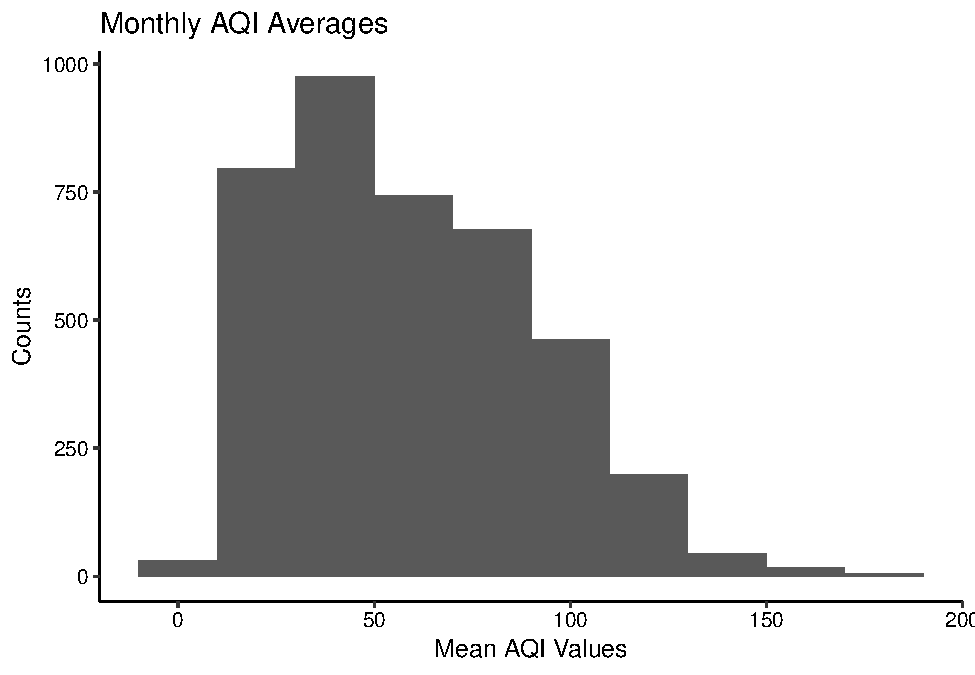
\includegraphics{Roth_ENV872_Project_files/figure-latex/exploratory graph1-1.pdf}
\caption{Histogram of monthly AQI averages for all sites 1980-2018}
\end{figure}

\begin{figure}
\centering
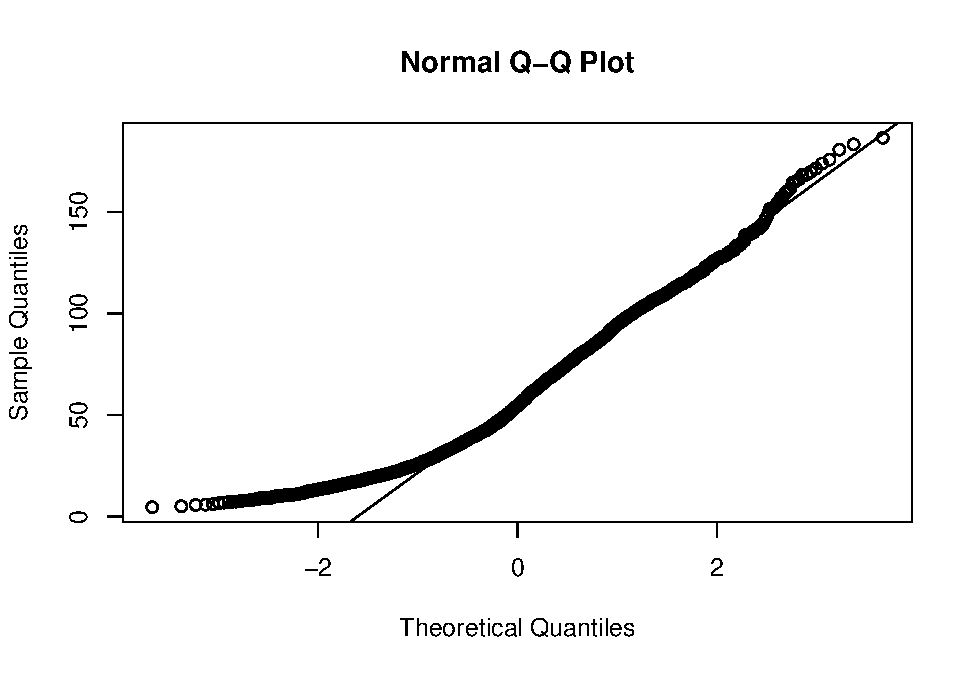
\includegraphics{Roth_ENV872_Project_files/figure-latex/exploratory graph2-1.pdf}
\caption{Q-Q plot of monthly AQI averages for all sites 1980-2018}
\end{figure}

\begin{figure}
\centering
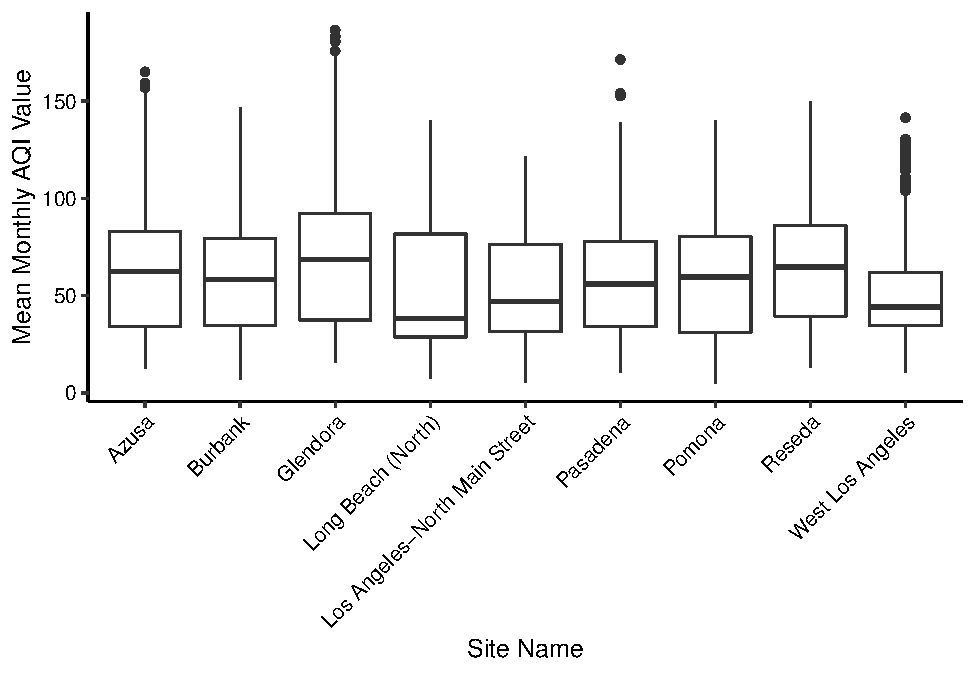
\includegraphics{Roth_ENV872_Project_files/figure-latex/exploratory graph3-1.pdf}
\caption{Boxplot of monthly AQI averages for each site 1980-2018}
\end{figure}

\newpage

\section{Analysis}\label{analysis}

I ran a series of Mann-Kendall and Pettitt tests to find where the
statistically significant breakpoints were in the monthly summary data.
First, the Mann-Kendall test on the entire data set showed that there
was a significant negative trend for all of the years of ozone data (z =
-27.304, n = 3951, p-value \textless{} 2.2e-16). Next, the Pettitt test
on the entire data set showed that there was a break point at the year
1995 (U = 2454000, p-value \textless{} 2.2e-16). Mann-Kendall tests on
the data before and after the break point showed a significant negative
trend between 1980 and 1995 (z = -5.1171, n = 1499, p-value = 3.102e-07)
and significant positive trend from 1995 to 2018 (z = 7.2036, n = 2452,
p-value = 5.863e-13). A second Pettitt test showed another break point
in 2011 (U = 227390, p-value = 1.462e-09). The Mann-Kendall tests showed
there was not a significant trend from 1995 to 2011 (z = 1.8849, n =
1790, p-value = 0.05945) and a significant positive trend from 2011 to
2018 (z = 2.9277, n = 662, p-value = 0.003415). A third Pettitt test
showed one more break point at 2016 (U = 18004, p-value = 0.002478). The
Mann-Kendall tests showed there was a significant positive trend from
2011 to 2016 (z = 2.618, n = 486, p-value = 0.008846), and no
significant trend between 2016 and 2019 (z = -0.83549, n = 176, p-value
= 0.4034). A final Pettitt test was run on the remaining section to
ensure there were no more statistically significant break points in the
data remaining (U* = 1387, p-value = 0.2436).

\begin{Shaded}
\begin{Highlighting}[]
\KeywordTok{mk.test}\NormalTok{(O3_total_month_processed}\OperatorTok{$}\NormalTok{MeanAQI)}
\end{Highlighting}
\end{Shaded}

\begin{verbatim}
## 
##  Mann-Kendall trend test
## 
## data:  O3_total_month_processed$MeanAQI
## z = -27.304, n = 3951, p-value < 2.2e-16
## alternative hypothesis: true S is not equal to 0
## sample estimates:
##             S          varS           tau 
## -2.260713e+06  6.855566e+09 -2.897297e-01
\end{verbatim}

\begin{Shaded}
\begin{Highlighting}[]
\KeywordTok{pettitt.test}\NormalTok{(O3_total_month_processed}\OperatorTok{$}\NormalTok{MeanAQI) }\CommentTok{#change point at 1500}
\end{Highlighting}
\end{Shaded}

\begin{verbatim}
## 
##  Pettitt's test for single change-point detection
## 
## data:  O3_total_month_processed$MeanAQI
## U* = 2454000, p-value < 2.2e-16
## alternative hypothesis: two.sided
## sample estimates:
## probable change point at time K 
##                            1500
\end{verbatim}

\begin{Shaded}
\begin{Highlighting}[]
\KeywordTok{mk.test}\NormalTok{(O3_total_month_processed}\OperatorTok{$}\NormalTok{MeanAQI[}\DecValTok{1}\OperatorTok{:}\DecValTok{1499}\NormalTok{])}
\end{Highlighting}
\end{Shaded}

\begin{verbatim}
## 
##  Mann-Kendall trend test
## 
## data:  O3_total_month_processed$MeanAQI[1:1499]
## z = -5.1171, n = 1499, p-value = 3.102e-07
## alternative hypothesis: true S is not equal to 0
## sample estimates:
##             S          varS           tau 
## -9.904400e+04  3.746245e+08 -8.822030e-02
\end{verbatim}

\begin{Shaded}
\begin{Highlighting}[]
\KeywordTok{mk.test}\NormalTok{(O3_total_month_processed}\OperatorTok{$}\NormalTok{MeanAQI[}\DecValTok{1500}\OperatorTok{:}\DecValTok{3951}\NormalTok{])}
\end{Highlighting}
\end{Shaded}

\begin{verbatim}
## 
##  Mann-Kendall trend test
## 
## data:  O3_total_month_processed$MeanAQI[1500:3951]
## z = 7.2036, n = 2452, p-value = 5.863e-13
## alternative hypothesis: true S is not equal to 0
## sample estimates:
##            S         varS          tau 
## 2.916390e+05 1.639020e+09 9.706037e-02
\end{verbatim}

\begin{Shaded}
\begin{Highlighting}[]
\KeywordTok{pettitt.test}\NormalTok{(O3_total_month_processed}\OperatorTok{$}\NormalTok{MeanAQI[}\DecValTok{1500}\OperatorTok{:}\DecValTok{3951}\NormalTok{]) }\CommentTok{#change point at 1790 +1500}
\end{Highlighting}
\end{Shaded}

\begin{verbatim}
## 
##  Pettitt's test for single change-point detection
## 
## data:  O3_total_month_processed$MeanAQI[1500:3951]
## U* = 227390, p-value = 1.462e-09
## alternative hypothesis: two.sided
## sample estimates:
## probable change point at time K 
##                            1790
\end{verbatim}

\begin{Shaded}
\begin{Highlighting}[]
\KeywordTok{mk.test}\NormalTok{(O3_total_month_processed}\OperatorTok{$}\NormalTok{MeanAQI[}\DecValTok{1500}\OperatorTok{:}\DecValTok{3289}\NormalTok{])}
\end{Highlighting}
\end{Shaded}

\begin{verbatim}
## 
##  Mann-Kendall trend test
## 
## data:  O3_total_month_processed$MeanAQI[1500:3289]
## z = 1.8849, n = 1790, p-value = 0.05945
## alternative hypothesis: true S is not equal to 0
## sample estimates:
##            S         varS          tau 
## 4.760300e+04 6.377932e+08 2.973262e-02
\end{verbatim}

\begin{Shaded}
\begin{Highlighting}[]
\KeywordTok{mk.test}\NormalTok{(O3_total_month_processed}\OperatorTok{$}\NormalTok{MeanAQI[}\DecValTok{3290}\OperatorTok{:}\DecValTok{3951}\NormalTok{])}
\end{Highlighting}
\end{Shaded}

\begin{verbatim}
## 
##  Mann-Kendall trend test
## 
## data:  O3_total_month_processed$MeanAQI[3290:3951]
## z = 2.9277, n = 662, p-value = 0.003415
## alternative hypothesis: true S is not equal to 0
## sample estimates:
##            S         varS          tau 
## 1.664200e+04 3.230810e+07 7.606989e-02
\end{verbatim}

\begin{Shaded}
\begin{Highlighting}[]
\KeywordTok{pettitt.test}\NormalTok{(O3_total_month_processed}\OperatorTok{$}\NormalTok{MeanAQI[}\DecValTok{3290}\OperatorTok{:}\DecValTok{3951}\NormalTok{]) }\CommentTok{#change point at 3290+ 243}
\end{Highlighting}
\end{Shaded}

\begin{verbatim}
## 
##  Pettitt's test for single change-point detection
## 
## data:  O3_total_month_processed$MeanAQI[3290:3951]
## U* = 18004, p-value = 0.002478
## alternative hypothesis: two.sided
## sample estimates:
## probable change point at time K 
##                             243
\end{verbatim}

\begin{Shaded}
\begin{Highlighting}[]
\KeywordTok{mk.test}\NormalTok{(O3_total_month_processed}\OperatorTok{$}\NormalTok{MeanAQI[}\DecValTok{3290}\OperatorTok{:}\DecValTok{3775}\NormalTok{])}
\end{Highlighting}
\end{Shaded}

\begin{verbatim}
## 
##  Mann-Kendall trend test
## 
## data:  O3_total_month_processed$MeanAQI[3290:3775]
## z = 2.618, n = 486, p-value = 0.008846
## alternative hypothesis: true S is not equal to 0
## sample estimates:
##            S         varS          tau 
## 9.365000e+03 1.279379e+07 7.946947e-02
\end{verbatim}

\begin{Shaded}
\begin{Highlighting}[]
\KeywordTok{mk.test}\NormalTok{(O3_total_month_processed}\OperatorTok{$}\NormalTok{MeanAQI[}\DecValTok{3776}\OperatorTok{:}\DecValTok{3951}\NormalTok{])}
\end{Highlighting}
\end{Shaded}

\begin{verbatim}
## 
##  Mann-Kendall trend test
## 
## data:  O3_total_month_processed$MeanAQI[3776:3951]
## z = -0.83549, n = 176, p-value = 0.4034
## alternative hypothesis: true S is not equal to 0
## sample estimates:
##             S          varS           tau 
## -6.540000e+02  6.108627e+05 -4.247305e-02
\end{verbatim}

\begin{Shaded}
\begin{Highlighting}[]
\KeywordTok{pettitt.test}\NormalTok{(O3_total_month_processed}\OperatorTok{$}\NormalTok{MeanAQI[}\DecValTok{3776}\OperatorTok{:}\DecValTok{3951}\NormalTok{]) }\CommentTok{#change point not significant}
\end{Highlighting}
\end{Shaded}

\begin{verbatim}
## 
##  Pettitt's test for single change-point detection
## 
## data:  O3_total_month_processed$MeanAQI[3776:3951]
## U* = 1387, p-value = 0.2436
## alternative hypothesis: two.sided
## sample estimates:
## probable change point at time K 
##                             114
\end{verbatim}

I then Ran a Seasonal Mann-Kendall test on the entire data set to
determine if there was any statistically significant differences between
subsets of each year. First, I ran a seasonal test with a frequency of
4, representing the 3 months of each annual season. The results showed a
statistically significant difference between all four seasons
(p\textless{}0.01). Next, I ran a seasonal test with a frequency of 12,
representing all 12 months out of the year. The results showed a
statistically significant difference between each of the 12 months out
of the year (p\textless{}0.01).

\begin{Shaded}
\begin{Highlighting}[]
\NormalTok{O3_alldata_processed}\OperatorTok{$}\NormalTok{DAILY_AQI_VALUE <-}\StringTok{ }\KeywordTok{as.numeric}\NormalTok{(O3_alldata_processed}\OperatorTok{$}\NormalTok{DAILY_AQI_VALUE)}
\NormalTok{O3_alldata_processed_timeseries_season <-}\StringTok{ }\KeywordTok{ts}\NormalTok{(O3_alldata_processed}\OperatorTok{$}\NormalTok{DAILY_AQI_VALUE,}
                                \DataTypeTok{start =} \KeywordTok{c}\NormalTok{(}\DecValTok{1980}\NormalTok{, }\DecValTok{1}\NormalTok{) ,}\DataTypeTok{frequency =} \DecValTok{4}\NormalTok{)}

\NormalTok{O3_alldata_season_smk <-}\StringTok{ }\KeywordTok{smk.test}\NormalTok{(O3_alldata_processed_timeseries_season)}
\KeywordTok{summary}\NormalTok{(O3_alldata_season_smk)}
\end{Highlighting}
\end{Shaded}

\begin{verbatim}
## 
##  Seasonal Mann-Kendall trend test (Hirsch-Slack test)
## 
## data: O3_alldata_processed_timeseries_season
## alternative hypothesis: two.sided
## 
## Statistics for individual seasons
## 
## H0
##                           S         varS    tau      z   Pr(>|z|)    
## Season 1:   S = 0 -11299544 2.772015e+12 -0.027 -6.787 1.1467e-11 ***
## Season 2:   S = 0 -11753598 2.772032e+12 -0.028 -7.059 1.6715e-12 ***
## Season 3:   S = 0 -11894469 2.772026e+12 -0.028 -7.144 9.0600e-13 ***
## Season 4:   S = 0 -10999066 2.772012e+12 -0.026 -6.606 3.9405e-11 ***
## ---
## Signif. codes:  0 '***' 0.001 '**' 0.01 '*' 0.05 '.' 0.1 ' ' 1
\end{verbatim}

\begin{Shaded}
\begin{Highlighting}[]
\NormalTok{O3_alldata_processed_timeseries_month <-}\StringTok{ }\KeywordTok{ts}\NormalTok{(O3_alldata_processed}\OperatorTok{$}\NormalTok{DAILY_AQI_VALUE,}
                                \DataTypeTok{start =} \KeywordTok{c}\NormalTok{(}\DecValTok{1980}\NormalTok{, }\DecValTok{1}\NormalTok{) ,}\DataTypeTok{frequency =} \DecValTok{12}\NormalTok{)}

\NormalTok{O3_alldata_month_smk <-}\StringTok{ }\KeywordTok{smk.test}\NormalTok{(O3_alldata_processed_timeseries_month)}
\KeywordTok{summary}\NormalTok{(O3_alldata_month_smk)}
\end{Highlighting}
\end{Shaded}

\begin{verbatim}
## 
##  Seasonal Mann-Kendall trend test (Hirsch-Slack test)
## 
## data: O3_alldata_processed_timeseries_month
## alternative hypothesis: two.sided
## 
## Statistics for individual seasons
## 
## H0
##                           S         varS    tau      z   Pr(>|z|)    
## Season 1:   S = 0  -1431794 102687255634 -0.030 -4.468 7.8921e-06 ***
## Season 2:   S = 0  -1417358 102687481705 -0.030 -4.423 9.7323e-06 ***
## Season 3:   S = 0  -1518742 102688379095 -0.032 -4.739 2.1436e-06 ***
## Season 4:   S = 0  -1316975 102686618118 -0.028 -4.110 3.9601e-05 ***
## Season 5:   S = 0  -1012104 102688613953 -0.021 -3.158 0.00158652  **
## Season 6:   S = 0  -1201587 102688467008 -0.026 -3.750 0.00017706 ***
## Season 7:   S = 0  -1306967 102687768801 -0.028 -4.079 4.5319e-05 ***
## Season 8:   S = 0  -1150782 102689041525 -0.024 -3.591 0.00032925 ***
## Season 9:   S = 0  -1320892 102656313482 -0.028 -4.123 3.7457e-05 ***
## Season 10:   S = 0 -1298046 102658010792 -0.028 -4.051 5.0936e-05 ***
## Season 11:   S = 0 -1135191 102657128173 -0.024 -3.543 0.00039557 ***
## Season 12:   S = 0 -1197109 102655990485 -0.025 -3.736 0.00018675 ***
## ---
## Signif. codes:  0 '***' 0.001 '**' 0.01 '*' 0.05 '.' 0.1 ' ' 1
\end{verbatim}

Finally, since the data was not normally distributed, I ran a
Kruskal-Wallis test to determine if there was a significant difference
in Ozone concentration between each site. The results of the test showed
that there is a significant difference between the monthly averaged AQI
values for each site between 1980 and 2018 (Kruskal-Wallis chi-squared =
102.21, df = 8, p-value \textless{} 2.2e-16).

\begin{Shaded}
\begin{Highlighting}[]
\NormalTok{O3_total_month_processed}\OperatorTok{$}\NormalTok{Site.Name <-}\StringTok{ }\KeywordTok{as.factor}\NormalTok{(O3_total_month_processed}\OperatorTok{$}\NormalTok{Site.Name)}
\KeywordTok{kruskal.test}\NormalTok{(O3_total_month_processed}\OperatorTok{$}\NormalTok{MeanAQI, O3_total_month_processed}\OperatorTok{$}\NormalTok{Site.Name) }
\end{Highlighting}
\end{Shaded}

\begin{verbatim}
## 
##  Kruskal-Wallis rank sum test
## 
## data:  O3_total_month_processed$MeanAQI and O3_total_month_processed$Site.Name
## Kruskal-Wallis chi-squared = 102.21, df = 8, p-value < 2.2e-16
\end{verbatim}

Figure 4 shows the summarized monthly AQI values by year. The green
portion of the graph indicates ``Good'' levels of trophospheric ozone,
the yellow portion ``Moderate'' levels, the orange portion ``Unhealthy
for sensitive groups'', and the red portion ``Unhealthy''. The blue
dashed lines indicate the break points determined by the Pettitt tests.

\begin{figure}
\centering
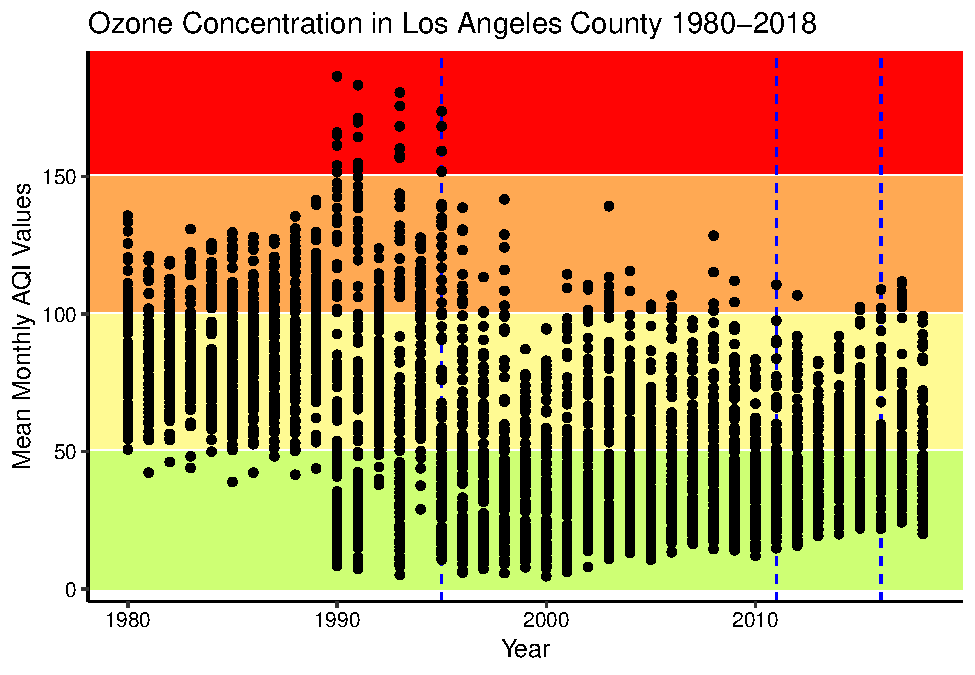
\includegraphics{Roth_ENV872_Project_files/figure-latex/plot data with break points-1.pdf}
\caption{Monthly AQI averages from 1980 to 2018 with break points}
\end{figure}

Figure 5 shows the summarized monthly AQI values by year and colored by
month. As noted by Sillman, it is expected that the highest ozone levels
will be in the hottest months, and the lowest ozone levels will be in
the cooler months. This is clearly seen after 1990 with the blue-green
colors having higher ozone levels each year, and the yellow and purple
colors having lower ozone levels each year. Between 1980 and 1990, there
is not as clear of a distinction between the months and levels of ozone.

\begin{figure}
\centering
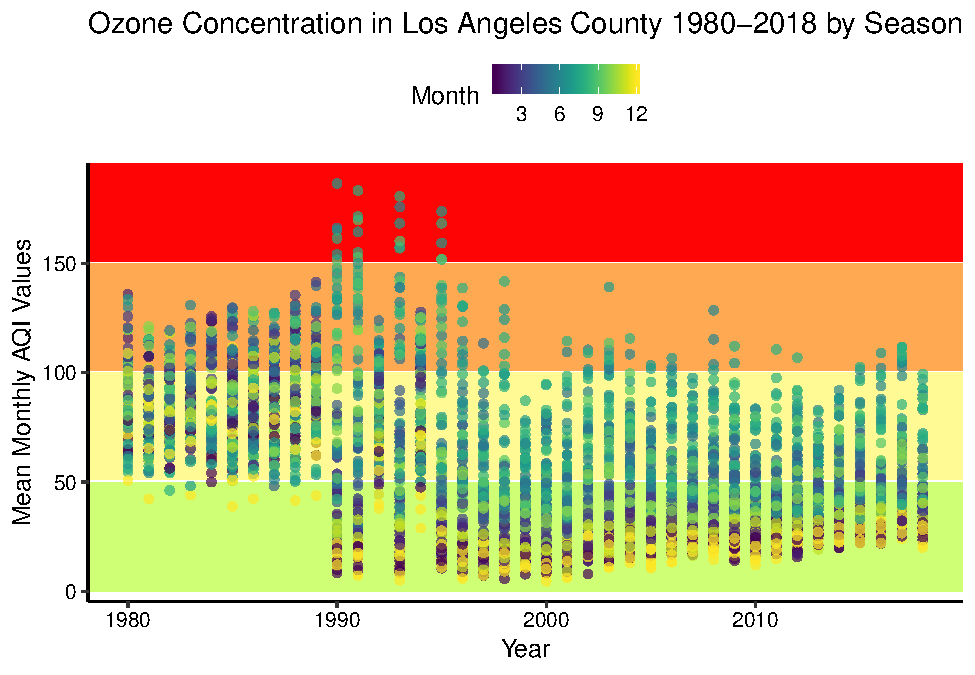
\includegraphics{Roth_ENV872_Project_files/figure-latex/plot data with seasons-1.pdf}
\caption{Monthly AQI averages from 1980 to 2018 by season}
\end{figure}

Figures 6-10 show the total daily AQI values for each site in the years
1980, 1990, 2000, 2010, and 2018. From 1980 to 2000, it is easy to see
that ozone is decreasing for each site over time. It seems that for some
of the sites between 2000 and 2010 the ozone levels seem to have more
concentrated AQI values at lower levels with some extreme events as
outliers, but the mean AQI values remain fairly constant. Locations more
inland like Reseda, Azusa, Burbank, Glendora, and Pasadena have higher
AQI values than sites closer to the coast such as West Los Angeles and
Los Angeles-North Main Street.

\begin{figure}
\centering
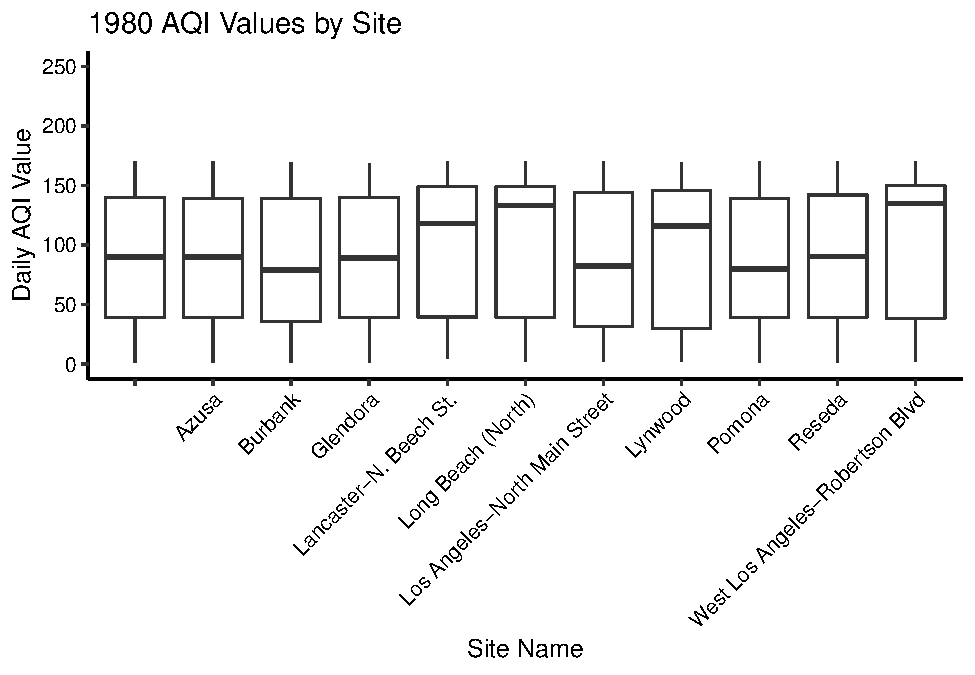
\includegraphics{Roth_ENV872_Project_files/figure-latex/box plot 1-1.pdf}
\caption{Boxplot of 1980 AQI values by site}
\end{figure}

\begin{verbatim}
## Warning: Removed 17 rows containing non-finite values (stat_boxplot).
\end{verbatim}

\begin{figure}
\centering
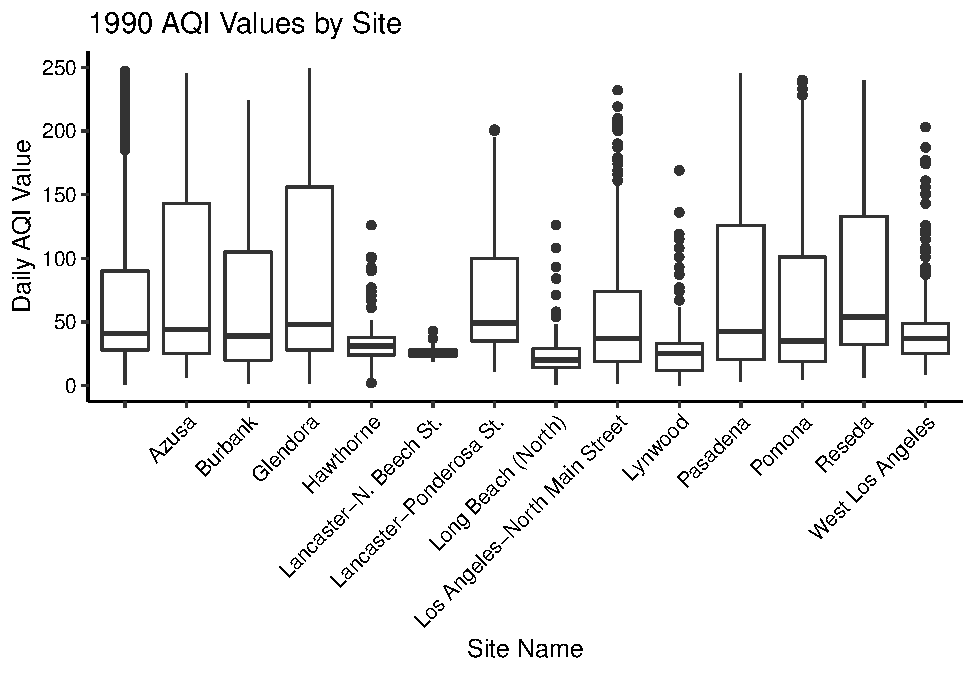
\includegraphics{Roth_ENV872_Project_files/figure-latex/box plot 2-1.pdf}
\caption{Boxplot of 1990 AQI values by site}
\end{figure}

\begin{figure}
\centering
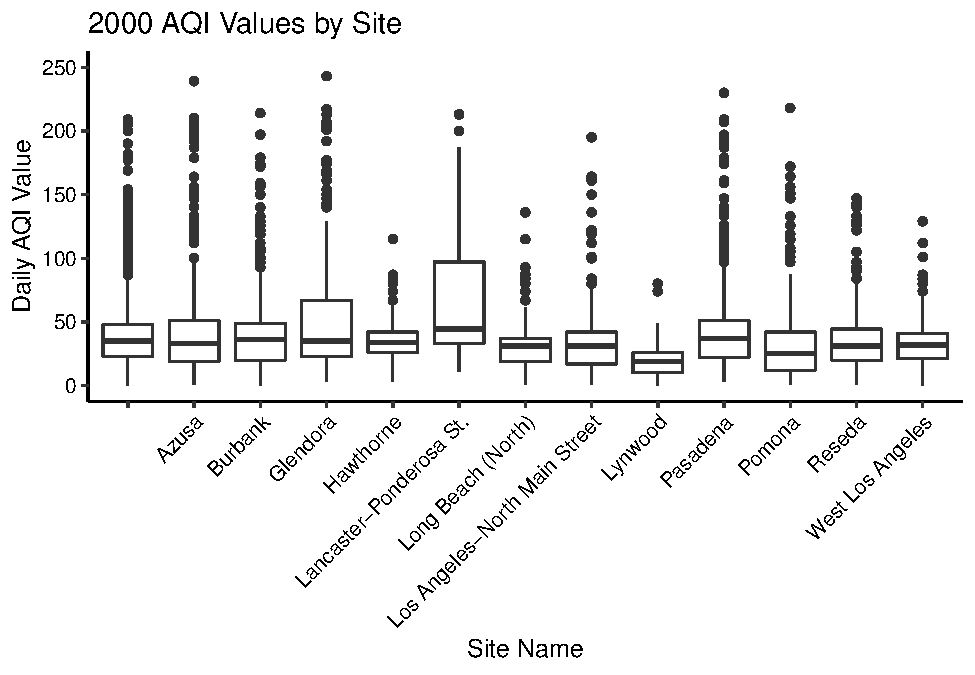
\includegraphics{Roth_ENV872_Project_files/figure-latex/box plot 3-1.pdf}
\caption{Boxplot of 2000 AQI values by site}
\end{figure}

\begin{figure}
\centering
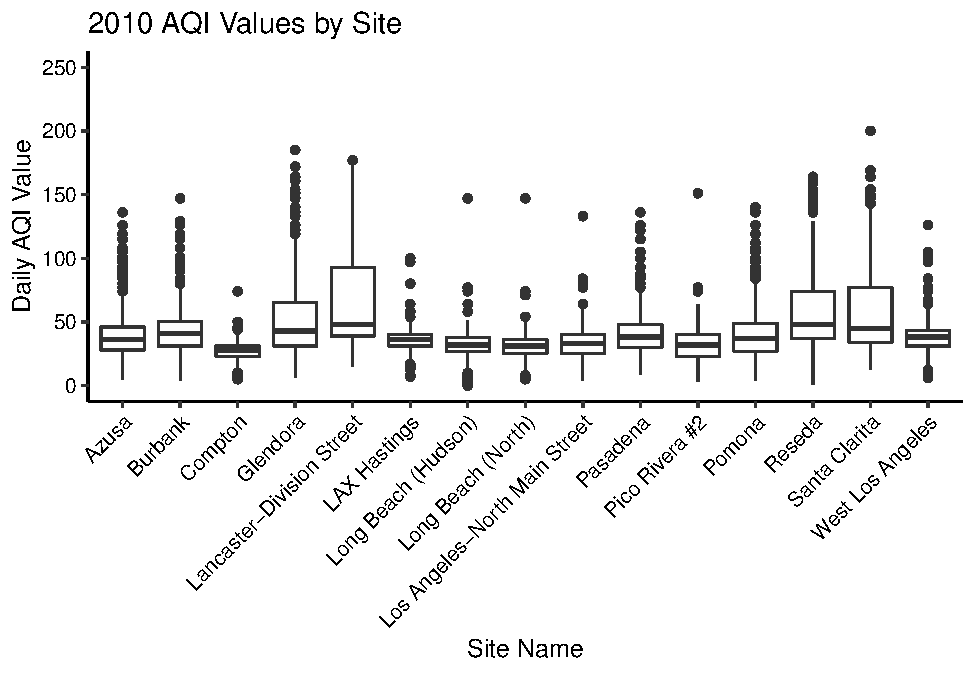
\includegraphics{Roth_ENV872_Project_files/figure-latex/box plot 4-1.pdf}
\caption{Boxplot of 2010 AQI values by site}
\end{figure}

\begin{figure}
\centering
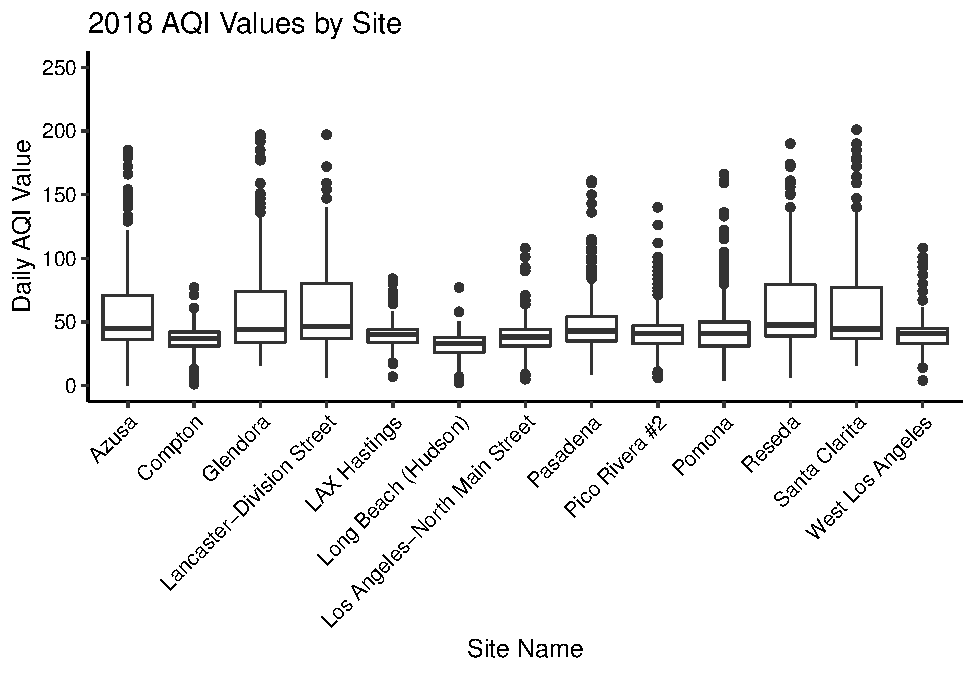
\includegraphics{Roth_ENV872_Project_files/figure-latex/box plot 5-1.pdf}
\caption{Boxplot of 2018 AQI values by site}
\end{figure}

\newpage

\section{Summary and Conclusions}\label{summary-and-conclusions}

This analysis shows that average ozone levels as well as the intensity
of extreme ozone events have decreased overall in Los Angeles County
between 1980 and 2018. The implementation of more stringent ozone
regulations by way of lowering the NAAQS levels for tropospheric ozone
and higher standards for automobile emissions put in place in 1990 as an
amendment to the Clean Air Act are likely the reason for this trend
(EPA, 2017). However, it also showed that there have been some
increasing average ozone levels since 2011. This may be due to
population growth in a city whose transportation is dominated by
personal automobiles as well as an increase in economic growth and
emissions following the Great Recession of 2008 (Peters et al., 2012).
This, combined with rising average annual temperatures as a result of
climate change, would likely result in higher levels of ozone throughout
the more recent years. Because vehicle emissions are such a large
contributor to tropospheric ozone and photochemical smog, increasing the
proportion of electric and hybrid vehicles owned and driven by Los
Angeles County residents could reduce this effect in the coming decades
in order to mitigate the impacts of climate change.

Additionally, there were found to be higher levels of ozone at inland
measurement sites compared to those closer to the coast. This could be
attributed to the unique geographic composition of Los Angeles County.
The daytime sea breeze blows smog away from the coast, where it is then
trapped by the surrounding mountain formations, leading to higher levels
of ozone around the inner edges of Los Angeles during the day (Lu \&
Turco, 1996). There were some irregularities in the data between 1980
and 1990, as seen by the lack of seasonality of the graphed data points
and the dramatic shift in the range of AQI values. This could
potentially be due to a change in collection methodology around 1990,
allowing for more accurate ozone measurements to be taken, but more
research into that anomaly is required.

\newpage

\section{Sources}\label{sources}

U.S. Environmental Protection Agency (EPA). (2017). Clean Air Act
Overview. Retrieved from
\url{https://www.epa.gov/clean-air-act-overview/1990-clean-air-act-amendment-summary-title-i}

Haagen-Smit, A. J. (1952). Chemistry and physiology of Los Angeles smog.
Industrial \& Engineering Chemistry, 44(6), 1342-1346.

Lu, R., \& Turco, R. P. (1996). Ozone distributions over the Los Angeles
basin: Three-dimensional simulations with the SMOG model. Atmospheric
Environment, 30(24), 4155-4176.

Peters, G. P., Marland, G., Le Quéré, C., Boden, T., Canadell, J. G., \&
Raupach, M. R. (2012). Rapid growth in CO 2 emissions after the
2008--2009 global financial crisis. Nature Climate Change, 2(1), 2.

Sillman, S. (2003). Overview: Tropospheric ozone, smog and ozone-NOx-VOC
sensitivity. Treatise on Geochemistry.


\end{document}
